\chapter{Diversité} \label{ch:DIV}

\section{Mesures et méthodologie}

L'objectif du travail est de quantifier l'impacte de la diversité sur la propagation de pandémies. Cette section est dédié à la prises de mesures avec des niveaux de diversité différents et d'en constater les résultats. Afin de ne pas trop complexifier le modèle au delà des simulations SIR, nous ne modifions que le paramètre de diversité, nombre de mouvements ainsi que la charge virale. D'autres paramètres du modèle pourraient être étudié mais ce chapitre ne les explore pas.\\

Toutes les musures de diversité ont été effectuées sur des systèmes aux paramètres semblables. La taille des systèmes est définie à $1264\times 1264$ avec une population de $10^5$ individus, il s'agit de systèmes en densité $\frac{1}{16}$. Un exemple de fichier de configuration est donné ci-dessous.

\begin{minted}
	[
	frame=lines,
	framesep=2mm,
	baselinestretch=1.2,
	bgcolor=LightGray,
	fontsize=\footnotesize,
	linenos
	]
	{c++}
	TAILLE_SYSTEME = 1264
	NOMBRE_INDIVIDUS = 100000
	ITERATIONS = 5000
	RERUN_LIMIT = 100
	FAIL_SEUIL = 30
	GENOME_INIT_I = 0
	GENOME_DIVERSITY_I = 8
	GENOME_INIT_AP = 0
	VITESSE_MUTATIONS_AP = 0
	CHARGE_VIRALE = 1
	PARAMETRE_FONCTION = 4
	CELLULE_AP = 0
	SURVIE_AP = 0
	NOMBRE_MOUVEMENT = 1
	PERFECT_MIX = true
	TEMPS_AVANT_IMMUNITE = 1
	IMMUNITE_MECANISME = true
	RESISTANCE_MECANISME = false
\end{minted}

L'exemple de fichier de configuration produit une simulation au mélange parfait avec une diversité de $8$. La configuration est similaire à celle d'une simulation SIR, la seule différence ici est l'ajout d'un paramètre de diversité non égal à $0$.\\

Toutes les simulations qui suivent se basent sur ce fichier de configuration mais avec quelques modifications.\\

Premièrement, le niveau de diversité varie d'une simulation à une autre. Les valeurs de diversité choisie sont : $4,8,16,32$. Pour rappel, une diversité de $x$ signifie que $x$ bits des génomes des individus seront complémentés et ceci alétoirement. Sans diversité les génomes des individus sont tous identiques.\\

Deuxièmement, le mode de mouvement ainsi que le nombre de mouvements varient. Seule la première simulation servant d'exemple utilise le mode de mouvement au mélange parfait, toutes les autres ont un nombre de mouvements défini. Les mouvements étudiés sont : $1,10,50$.\\

Finalement nous faisons varier le paramètre de charge virale (ici défini à 1). L'idée principale est de ralentir la propagation de pandémies en diminuant la contagion des agents pathogènes. Les simulations sont effectuée sur $4$ niveaux de charge virale : $0.25,0.5,0.75,1$\\

Un total de $64$ configurations de simulations sont étudiées et pour chacune de ces configuration nous effectuons $100$ simulations. L'exécution de $100$ simulations pour un ensemble de paramètres permet de calculer le taux d'événements pandémiques ainsi que de relever les caractéristiques des simulations qui ne font pas apparaitre de pandémie.

\section{Résultats}

Le premier résultat présenté est un exemple d'impacte de la diverstié sur une simulation qui déclanche une pandémie. La suite présente des statistiques sur les simulations incluant de la diversité qui n'ont pas développé de pandémie. En effet, nous nous intéressons tout particulièrement aux situations ou une pandémie est évitée. Les données relevées concernant ces simulations sont : le nombre maximum de contaminés simultanément, l'itération de ce maximum, l'itération de fin de simulations (lorsque plus aucun individu n'est contaminé) et finalement le taux de simulations qui ont développé une pandémie parmi les $100$ simulations pour chaque configuration.

\subsection{Mélange parfait}

Le document ne contient qu'une seule simulation à diversité non nulle et au mélange parfait. La raison pour laquelle cette voie n'est que peu explorée est parceque le mélange parfait est trop efficace pour la propagation de pandémies. Par conséquent les propagations sont beaucoup trop rapides comparé au ralentissement qu'offre la diversité.

\newpage

\begin{figure}[h]
	\centering
	\captionsetup{justification=centering}
	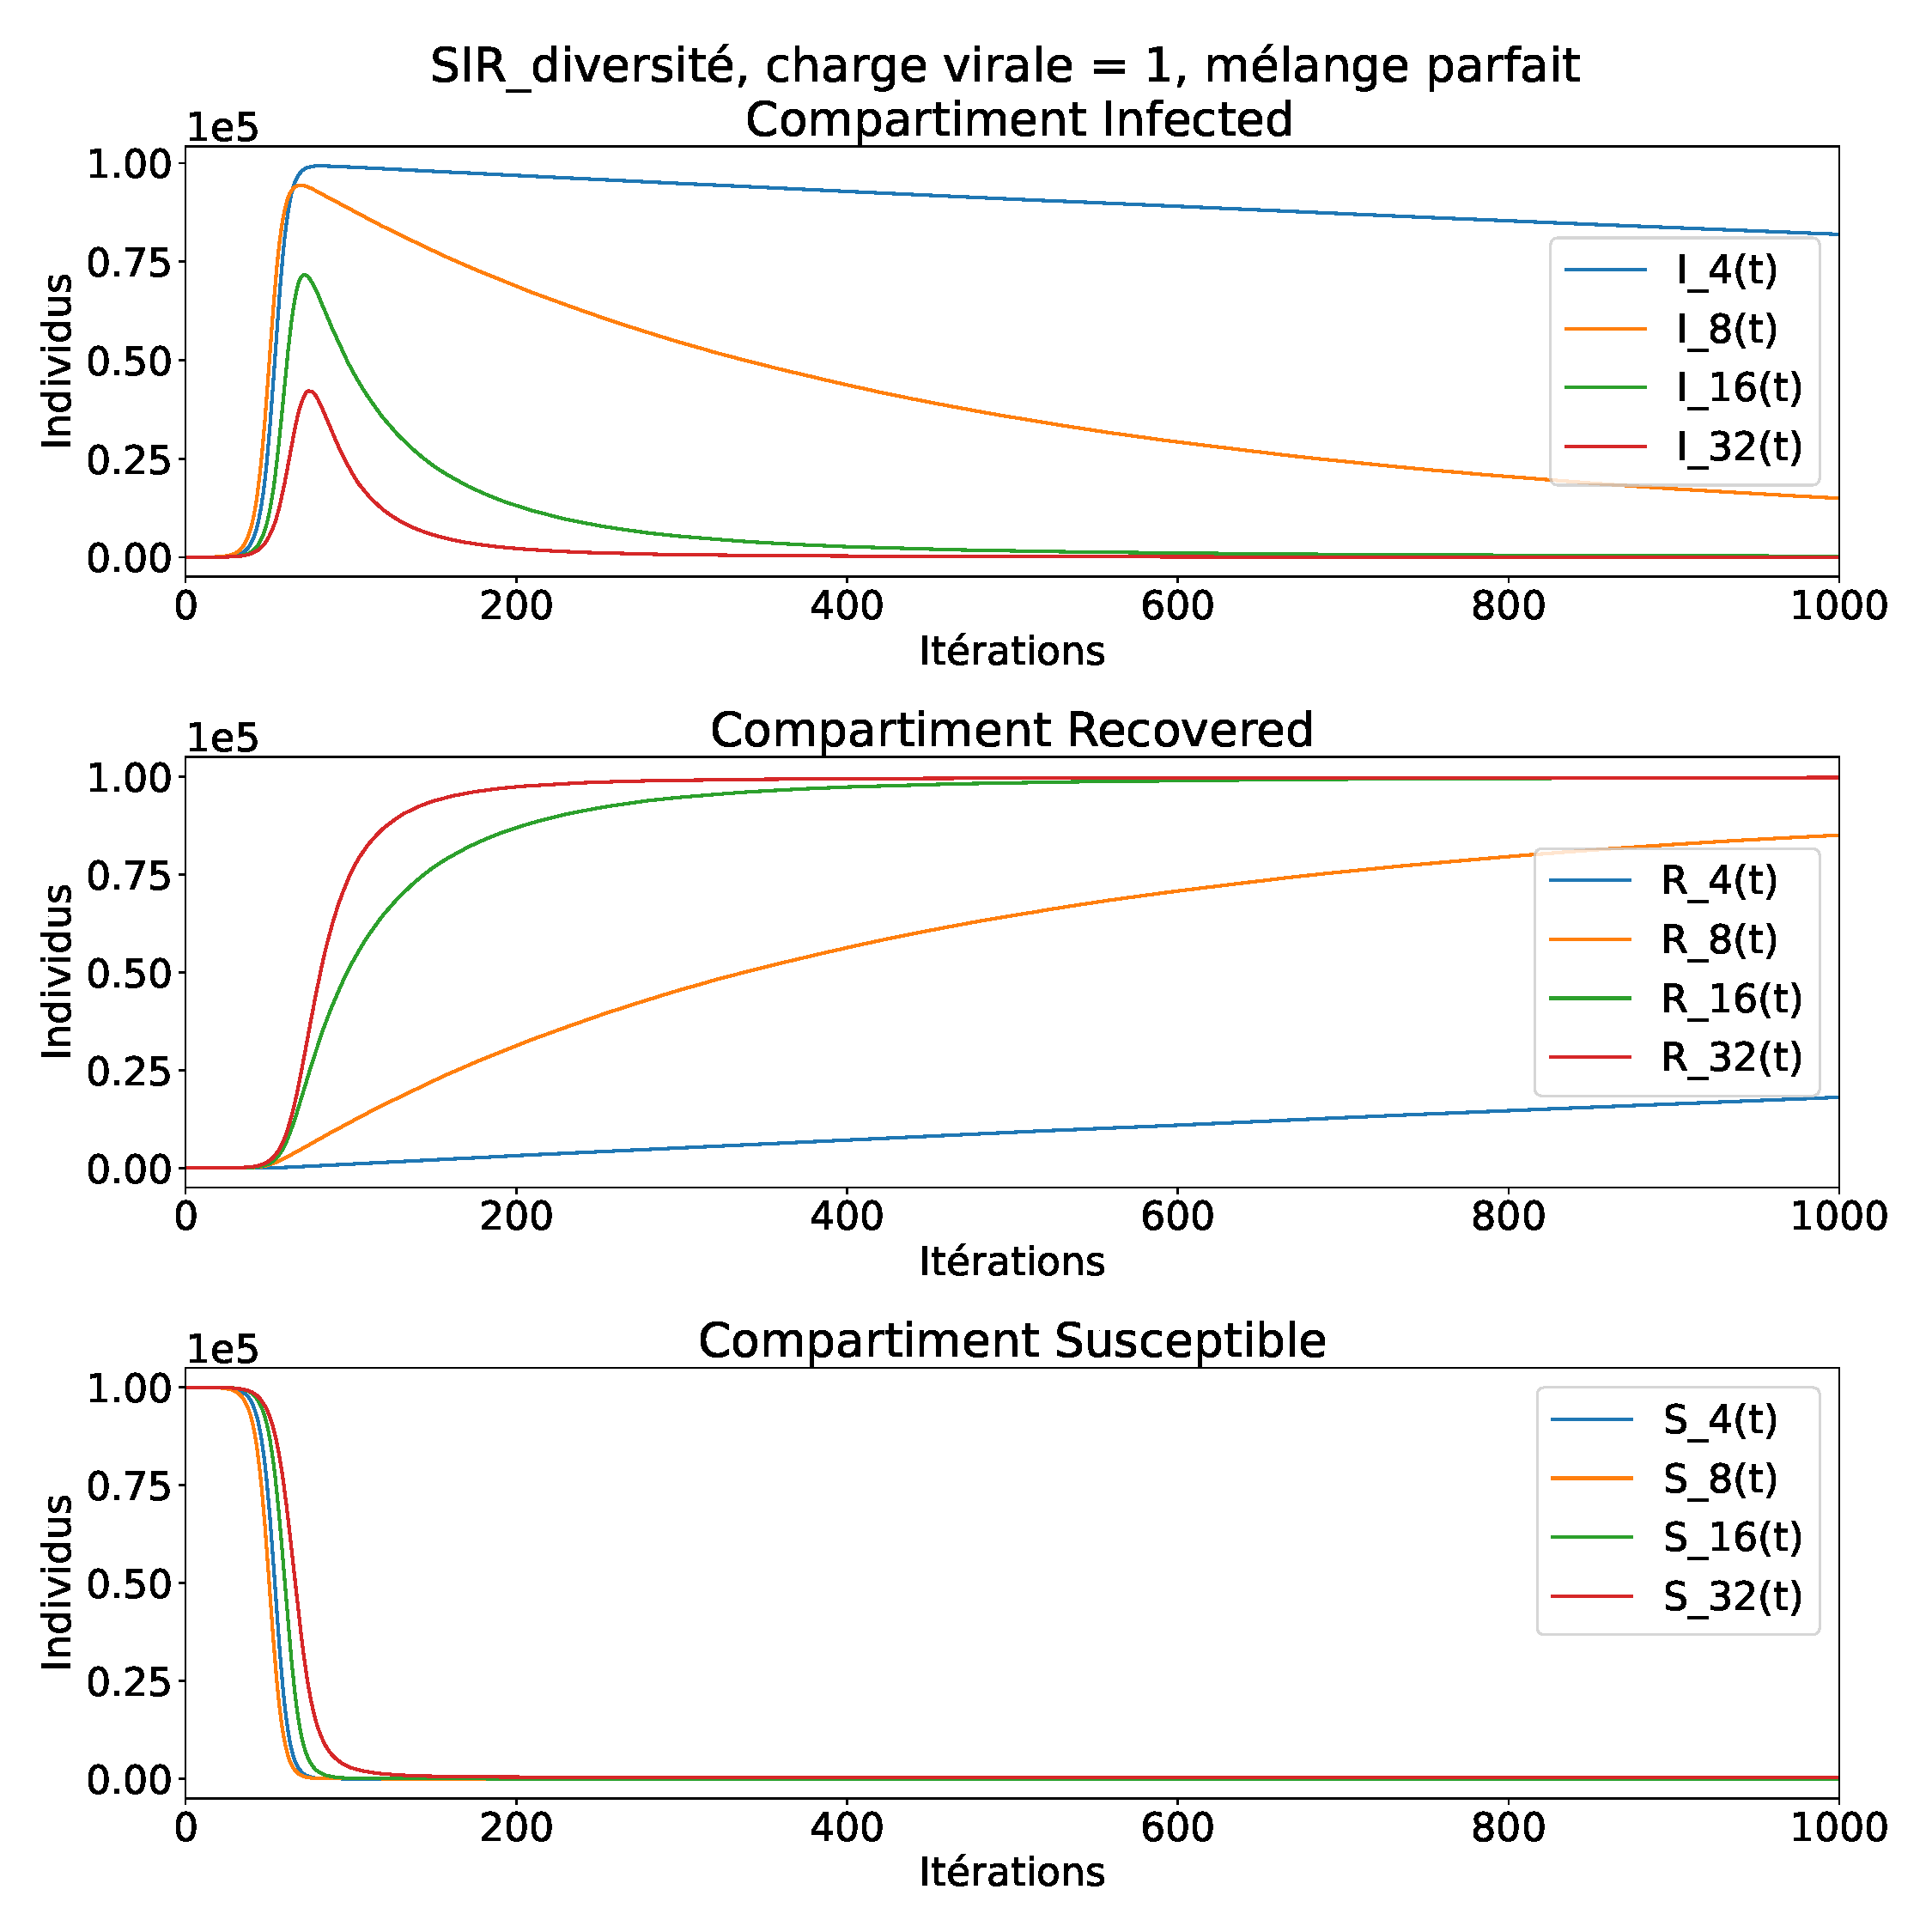
\includegraphics[width=.8\textwidth]{Images/SIR_diversite_mix.pdf}
	\caption[Impacte de la diversité]{Impacte de la diversité d'une population sur une simulation au mélange parfait avec $10^5$ individus et une densité de $1/16$. La première figure montre le compartiment $I$, le second le compartiment $R$ et le dernier le compartiement $S$. Chaque couleur de courbe fait référence à une simulation avec une certaine valeur de diversité notée dans la légende.}
\end{figure}

Les résultats des simulations au mélange parfait sont très similaire aux simulations SIR et ceci est dû au fait que l'impacte de la diversité est trop faible sur ces simulations. Pour pouvoir étudier l'impact de la diversité il est nécessaire de construire des systèmes plus progressifs dans la propagation des agents pathogènes.\\

Deux choses sont à noter à propos de cette figure. La première est que la propagation est beaucoup trop rapide comme nous pouvons le voir sur le compartiement $Susceptible$ qui tombe rapidement à $0$. Tous les individus sont déjà passés dans le compartiment $Infected$ très tôt dans la simulation. Par conséquent dans ces configurations la propagation de la pandémie est maximale car elle atteint rapidement $100\%$ de la population.\\

Le deuxième élément se produit dans une deuxième phase et décrit l'immunisation des individus. Comme nous l'avons déjà dit, tout les individus finissent contaminés très vite. A partir de là, les individus s'immunisent mais leur immunisation dépend de la compatibilité qu'ils ont avec leur agent pathogène. Le compartiment $Recovered$ montre la différence de vitesse des acquisitions d'immunisation parmi la population et il est assez clair qu'un plus grand niveau de diversité implique une immunisation générale plus rapide. Ceci est uiquement vrai parce que le génome initial des individu les rend très vulnérable au pathogène. Par conséquent, dans cette situation la diversité permet une meilleure immunisation de la population.

\subsection{Mouvements variable}

\setlength{\tabcolsep}{4pt}

\begin{table}[H]
	\centering
	\captionsetup{justification=centering}
	\caption[1]{2\label{tab:grid}}
	\begin{tabular}{@{\extracolsep{\fill} } c|| c| c| c|| c| c| c|| c| c| c|| c| c| c|}
		4    & \multicolumn{3}{|c||}{succès} & \multicolumn{3}{|c||}{max} & \multicolumn{3}{|c||}{it\_max} & \multicolumn{3}{|c|}{it\_fin}                                       \\
		\midrule
		     & 1 & 10 & 50 & 1 & 10 & 50 & 1 & 10 & 50 & 1 & 10 & 50 \\
		\midrule
		\midrule
		1    & 100\%  & 99\% & 99\% & nan & 1  & 1  & nan & 0  & 0  & nan & 1  & 1  \\
		\midrule
		0.75 & 100\% & 99\% & 100\% & nan & 1  & nan  & nan & 0  & nan  & nan & 17  & nan  \\
		\midrule
		0.5  & 100\% & 100\% & 100\% & nan & nan  & nan  & nan & nan  & nan  & nan & nan  & nan  \\
		\midrule
		0.25 & 100\% & 100\% & 100\% & nan & nan  & nan  & nan & nan  & nan  & nan & nan  & nan  \\
		\bottomrule
	\end{tabular}
\end{table}

\begin{table}[H]
	\centering
	\captionsetup{justification=centering}
	\caption[1]{2\label{tab:grid}}
	\begin{tabular}{@{\extracolsep{\fill} } c|| c| c| c|| c| c| c|| c| c| c|| c| c| c|}
		8    & \multicolumn{3}{|c||}{succès} & \multicolumn{3}{|c||}{max} & \multicolumn{3}{|c||}{it\_max} & \multicolumn{3}{|c|}{it\_fin}                                       \\
		\midrule
		     & 1 & 10 & 50 & 1 & 10 & 50 & 1 & 10 & 50 & 1 & 10 & 50 \\
		\midrule
		\midrule
		1    & 98\%  & 98\% & 99\% & 1 & 1  & 1  & 0 & 0  & 0  & 4.5 & 2  & 1  \\
		\midrule
		0.75 & 96\% & 98\% & 97\% & 1.25 & 1  & 1  & 6.25 & 0  & 0  & 21.25 & 3.5  & 6.67  \\
		\midrule
		0.5  & 95\% & 95\% & 98\% & 1.2 & 1  & 1  & 0.4 & 0  & 0  & 6.8 & 6.4  & 6.5  \\
		\midrule
		0.25 & 95\% & 95\% & 97\% & 1 & 1  & 1.34  & 0 & 0  & 5.34  & 20.4 & 17.8  & 19.67  \\
		\bottomrule
	\end{tabular}
\end{table}

\begin{table}[H]
	\centering
	\captionsetup{justification=centering}
	\caption[1]{2\label{tab:grid}}
	\begin{tabular}{@{\extracolsep{\fill} } c|| c| c| c|| c| c| c|| c| c| c|| c| c| c|}
		16    & \multicolumn{3}{|c||}{succès} & \multicolumn{3}{|c||}{max} & \multicolumn{3}{|c||}{it\_max} & \multicolumn{3}{|c|}{it\_fin}                                       \\
		\midrule
		     & 1 & 10 & 50 & 1 & 10 & 50 & 1 & 10 & 50 & 1 & 10 & 50 \\
		\midrule
		\midrule
		1    & 73\%  & 92\% & 99\% & 1.81 & 1.25  & 1  & 6.89 & 1.38  & 0  & 27.44 & 5.75  & 1  \\
		\midrule
		0.75 & 77\% & 84\% & 88\% & 1.26 & 1.06  & 1.08  & 1 & 1.06  & 1.17  & 13.96 & 8.31  & 6.08  \\
		\midrule
		0.5  & 65\% & 79\% & 80\% & 2.86 & 1.19  & 1.25  & 30.14 & 1.43  & 1.2  & 155.51 & 11.28  & 12.6  \\
		\midrule
		0.25 & 1\% & 68\% & 67\% & 24.92 & 1.53  & 1.09  & 728.27 & 5.38  & 2.12  & 633.56 & 22.63  & 10.88  \\
		\bottomrule
	\end{tabular}
\end{table}

\begin{table}[H]
	\centering
	\captionsetup{justification=centering}
	\caption[1]{2\label{tab:grid}}
	\begin{tabular}{@{\extracolsep{\fill} } c|| c| c| c|| c| c| c|| c| c| c|| c| c| c|}
		32    & \multicolumn{3}{|c||}{succès} & \multicolumn{3}{|c||}{max} & \multicolumn{3}{|c||}{it\_max} & \multicolumn{3}{|c|}{it\_fin}                                       \\
		\midrule
		     & 1 & 10 & 50 & 1 & 10 & 50 & 1 & 10 & 50 & 1 & 10 & 50 \\
		\midrule
		\midrule
		1    & 0\%  & 74\% & 99\% & 5.02 & 1.38  & 1  & 46.71 & 3.46  & 0  & 125.91 & 8.08  & 1  \\
		\midrule
		0.75 & 0\% & 62\% & 65\% & 4.05 & 1.42  & 1.23  & 25.06 & 1.89  & 1.23  & 98.96 & 8.97  & 5.69  \\
		\midrule
		0.5  & 0\% & 48\% & 56\% & 2.63 & 1.92  & 1.27  & 16.89 & 4.98  & 1.27  & 55.72 & 16.63  & 7.5  \\
		\midrule
		0.25 & 0\% & 0\% & 18\% & 2.64 & 5.76  & 2.37  & 29.4 & 68.39  & 11.45  & 66.28 & 170.05  & 31.18  \\
		\bottomrule
	\end{tabular}
\end{table}

\subsection{Conclusion des résultats}

Les résultats permettent d'observer l'impacte de la diversité sur les systèmes. Apparemment il n'y a pas d'impacte sur la propagation de la pandémie mais uniquement sur la vitesse d'immunisation des individus. Nous cherchions à observer des pandémies qui évoluaient jusqu'à un certain point et dissparaissait ensuite mais ce comportement n'est pas présent dans les mesures.\\

L'absence de ces événements est dû au fonctionnement du modèle et à la notion de diversité. Le problème est que dans le modèle, la diversité n'a aucun impacte sur le propagation de pandémie. Pour rappel, lorsqu'un individu sain est en contact avec un agent pathogène, l'individu devient contaminé et contagieux directement et ceci peu importe la diversité du système. Le seul effet de la diverstié est le fait que cet individu peut s'immuniser plus ou moins rapidement en fonction de cette diversité. Mais le problème est que la propagation se présente sous forme de vague, comme une onde. L'illustration ci-dessous illustre le phénomène.

\begin{figure}[h]
	\centering
	\captionsetup{justification=centering}
	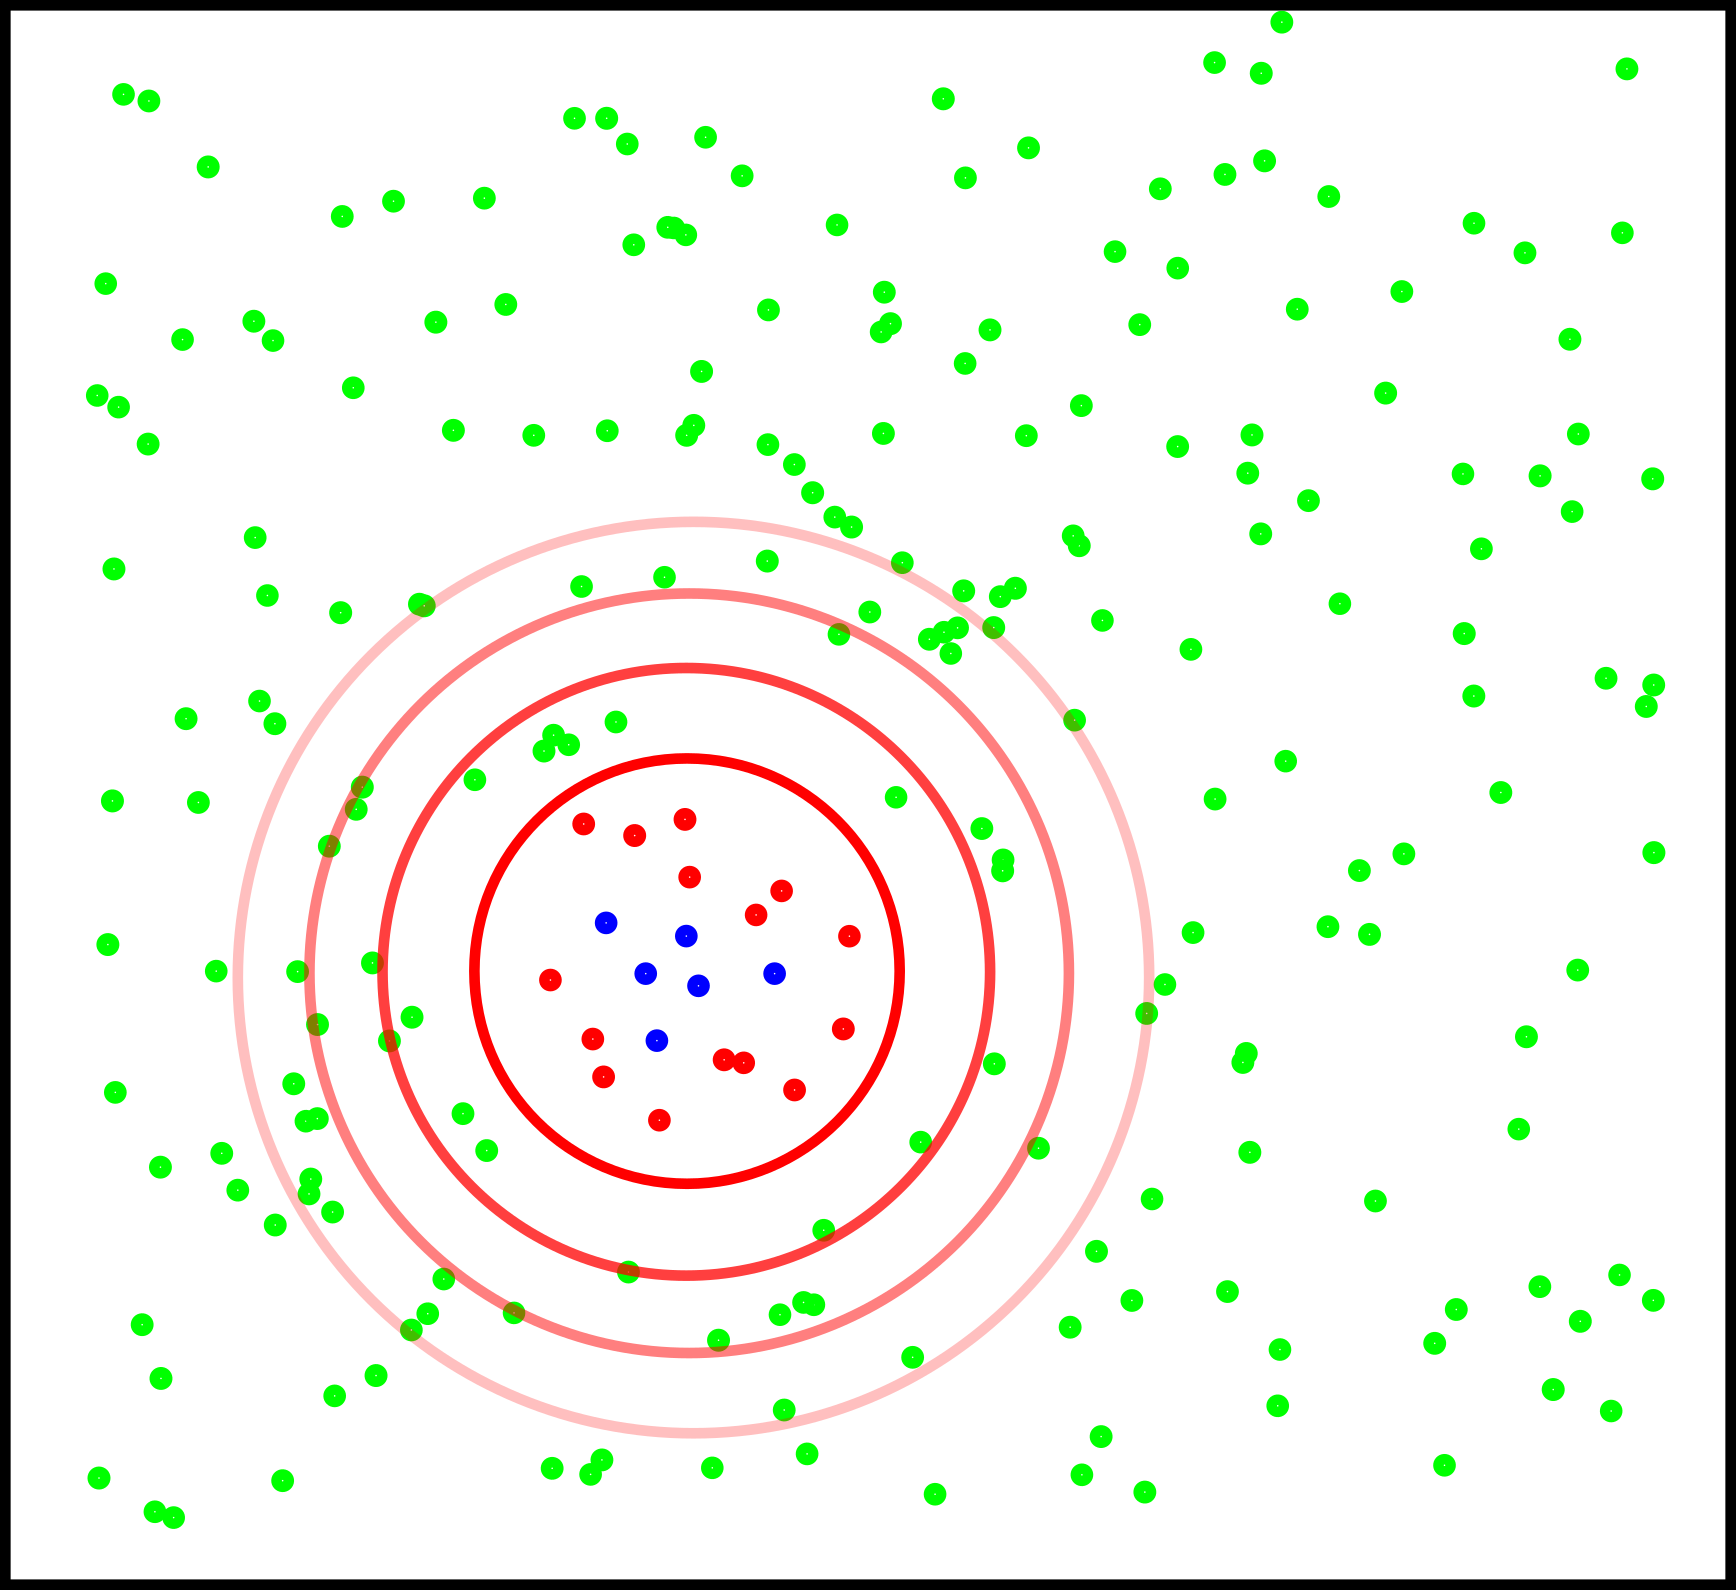
\includegraphics[width=.5\textwidth]{Images/vague_propagation.png}
	\caption{vague propagation}
\end{figure}

La figure montre la propagation d'une pandémie. En vert nous avons les individus sains, en bleu les individus immunisés et en rouge les individus contaminés. Les cercles représentent la propagation de la pandémie sous forme de vagues. Nous pourrion découper le processus en 3 zones distinctes et indépendantes. Le première est la zone centrale du cercle avec les individus immunisés. La seconde est la frontière entre les individus infectés et les sains donc la vague (cercle rouge) et finalement la troisième zone est le reste du système avec uniquement des individus sains.\\

D'après les résultats des simulations, la diversité n'impacte pas la propagation de la pandémie. En effet, la diversité permet l'immunisation plus rapide de la population donc l'apparition davantages de cercles bleus sur l'image. Le problème est que cette première zone est indépendante de la deuxième qui est la vague car cette dernière est beaucoup plus rapide que l'immunisation. Un individu fraichement contaminé propagera la pandémie bien avant qu'il ne s'immunise. Par conséquent, l'ampleur des immunisation n'impacte pas la propagation de la pandémie.\\

Donc la première zone n'affecte pas la vague mais qu'en est-il de la troisième zone ? En réalité la troisième zone est purement uniforme. Si une vague parvient à un moment donné à se propager dans la troisième zone alors elle le pourra jusqu'à contaminer tous les individus.\\

La rélexion mène donc à expliquer que une pandémie se propage soit complètement soit pas du tout.\\

En épidémiologie, le nombre de reproduction de base $R_0$ représente le nombre moyen de contaminations par un individu contaminé. Si ce taux est au dessous de $1$, cela signifie que la pandémie est mourante par contre si le taux est au dessus de $1$, la pandémie se propage.\\

Dans le modèle implémenté et d'après les mesures de diversité, une simulations ne peut pas avoir un $R_0$ qui varie. Cette valeur est fixe du début à la fin. Par conséquent, toutes les simulations au $R_0 < 1$ ne montrent aucune pandémie et au contraire toutes les simulations au $R_0 > 1$ finissent par contaminer tout le monde. Dans une situation réelle, des mesures sanitaires permettent de faire varier ce taux au cours de la propagation de la pendémie. Dans le modèle ce fonctionnement est non présent. Une autre chose n'est pas présente et donc impossible dans le modèle est l'effet d'immunité collective.\\

L'immunité collective est le fait le niveau d'immunité général est siffisemment élevé afin de faire passer le taux $R_0$ en dessous de $1$ et que la pandémie disparaisse. Ce phénomène peut s'obtenir par trois façons. La première est la vaccination, la seconde est l'immunité croisée et la troisième est une forme de résistance naturelle. Si nous reprenions la figure ci-dessus, l'immunité collective dans le modèle pourraient être obtenue d'une seule façon. Il faudrait pouroivr modifier l'état de la troisième zone (les parties du système non contaminés). Si au fil du temps nous pouvions vacciner des individus ou les immuniser en amont de la pandémie alors nous pourrions influencer le $R_0$ de la simulation mais le modèle n'inclut pas ces mécanismes. Par conséquent le $R_0$ reste constant dû à l'homogénéité de la troisième zone.


